% Copyright 2004 by Till Tantau <tantau@users.sourceforge.net>.
%
% In principle, this file can be redistributed and/or modified under
% the terms of the GNU Public License, version 2.

% However, this file is supposed to be a template to be modified
% for your own needs. For this reason, if you use this file as a
% template and not specifically distribute it as part of a another
% package/program, I grant the extra permission to freely copy and
% modify this file as you see fit and even to delete this copyright
% notice. 

\documentclass{beamer}

% There are many different themes available for Beamer. A comprehensive
% list with examples is given here:
% http://deic.uab.es/~iblanes/beamer_gallery/index_by_theme.html
% You can uncomment the themes below if you would like to use a different
% one:
%\usetheme{AnnArbor}
%\usetheme{Antibes}
%\usetheme{Bergen}
%\usetheme{Berkeley}
%\usetheme{Berlin}
%\usetheme{Boadilla}
%\usetheme{boxes}
%\usetheme{CambridgeUS}
%\usetheme{Copenhagen}
%\usetheme{Darmstadt}
%\usetheme{default}
%\usetheme{Frankfurt}
%\usetheme{Goettingen}
%\usetheme{Hannover}
%\usetheme{Ilmenau}
%\usetheme{JuanLesPins}
%\usetheme{Luebeck}
\usetheme{Madrid}
%\usetheme{Malmoe}
%\usetheme{Marburg}
%\usetheme{Montpellier}
%\usetheme{PaloAlto}
%\usetheme{Pittsburgh}
%\usetheme{Rochester}
%\usetheme{Singapore}
%\usetheme{Szeged}
%\usetheme{Warsaw}

\usecolortheme{beaver}
\usepackage{listings}
\usepackage{minted}

\setbeamertemplate{itemize/enumerate body begin}{\Large}
\setbeamertemplate{itemize/enumerate subbody begin}{\large}

\newcommand{\shellcmd}[1]{\\\indent\indent\texttt{\footnotesize\# #1}\\}

\title{MIT-IIT Robotics Program}

% A subtitle is optional and this may be deleted
%\subtitle{Optional Subtitle}

\author{Amartya Shankha Biswas}%\inst{1}}
% - Give the names in the same order as the appear in the paper.
% - Use the \inst{?} command only if the authors have different
%   affiliation.

% - Use the \inst command only if there are several affiliations.
% - Keep it simple, no one is interested in your street address.

\date{\today}
% - Either use conference name or its abbreviation.
% - Not really informative to the audience, more for people (including
%   yourself) who are reading the slides online

% Delete this, if you do not want the table of contents to pop up at
% the beginning of each subsection:
\AtBeginSubsection[]
{
  \begin{frame}<beamer>{Outline}
    \tableofcontents[currentsection,currentsubsection]
  \end{frame}
}

% Let's get started
\begin{document}

\begin{frame}
  \titlepage
\end{frame}

\begin{frame}{Outline}
  \tableofcontents`
  % You might wish to add the option [pausesections]
\end{frame}

% Section and subsections will appear in the presentation overview
% and table of contents.

\section{Recap}


\section{Logical Expressions}

\subsection{Booleans}
\begin{frame}[fragile]{Booleans}{A New Data Type}
    \begin{block}{}
        Booleans only have two possible values -- True or False
    \end{block}
    \vspace{1.5em}
    {\Large \textbf{Statement:} Schrodinger's cat is dead !}
    \begin{columns}[c]
        \column{.4\textwidth}
            \setbeamercolor{block title}{use=structure,fg=white,bg=green!35!black}
            \begin{block}{True}
            \begin{center}
                
\includegraphics[width=\linewidth]{images/dead_cat.jpg}
            \end{center}
            \end{block}
        \column{.4\textwidth}
            \setbeamercolor{block title}{use=structure,fg=white,bg=red!35!black}
            \begin{block}{False}
            \begin{center}
                
\includegraphics[width=\linewidth]{images/cat.jpg}
            \end{center}
            \end{block}
    \end{columns}
\end{frame}

\begin{frame}[fragile]{Booleans}{A New Data Type}
    \begin{itemize}
        \item In C++ we have a \textbf{bool} data-type
            \begin{minted}{c++}
                bool var = true;
            \end{minted}
        \item Actually stored as integer (\textbf{true} is 1 and \textbf{false} is 0)
        \pause
        \item In the other direction
            \begin{itemize}
                \item Zero value is \textbf{true}
                \item Non-Zero value is \textbf{false}
            \end{itemize}
    \end{itemize}
\end{frame}

\subsection{New Operators}
\begin{frame}[fragile]{Relational Operators}{}
    \begin{table}[]
    \centering
    \begin{tabular}{cccc}
    \hline
    \textbf{Operation}  & \textbf{Common Symbol} & \textbf{C++ Symbol} & \textbf{Expression} \\ \hline
    Equals              & $=$       & $==$  & $(a == b)           $ \\ \hline
    Not Equals          & $\not=$   & $!=$  & $(a \mathrel!= b)           $ \\ \hline
    Less Than           & $<$       & $<$   & $(a < b)    $ \\ \hline
    Greater Than        & $>$       & $>$   & $(a > b) $ \\ \hline
    Less Than Equals    & $\le$     & $<=$  & $(a <= b)   $ \\ \hline
    Greater Than Equals & $\ge$     & $>=$  & $(a >= b)$ \\ \hline
    \end{tabular}
    \end{table}
\end{frame}

\begin{frame}[fragile]{Logical Operators}{}
    \Large
    \begin{table}[]
    \centering
    \begin{tabular}{ccc}
    \hline
    \textbf{Operation} & \textbf{Symbol} & \textbf{Expression}        \\ \hline
    And                & $\&\&$          & $(a \mathrel!= b) \ \&\& \ (a \% 2 == 0)$ \\ \hline
    Or                 & $||$            & $(a > b) \ || \ (a / 2 > 4)$   \\ \hline
    Not                & $!$             & $!(a == b)$                \\ \hline
    \end{tabular}
    \end{table}
\end{frame}



\section{Conditionals}

\subsection{If Else Statements}
\begin{frame}[fragile]{If and Else}{}
    \begin{block}{}
        The \textbf{else} statement is optional.
    \end{block}
    \begin{minted}{c++}
        if (temperature >= 38)
            cout << "Buy an ice ceam cone" << endl;
        else
            cout << "Buy a lollipop" << endl;
    \end{minted}
    \begin{block}{}
        Must use a block (surrounded by curly braces) for more than one line.
    \end{block}
    \begin{minted}{c++}
        if (number_of_lines > 1) {
            cout << "More than one line.";
            cout << "Have to use a block.";
        }
        else{
            cout << "Curly braces are optional.";
        }
    \end{minted}
\end{frame}

\begin{frame}[fragile]{The \textbf{if...else if...else} Statement}{}
    \begin{center}
        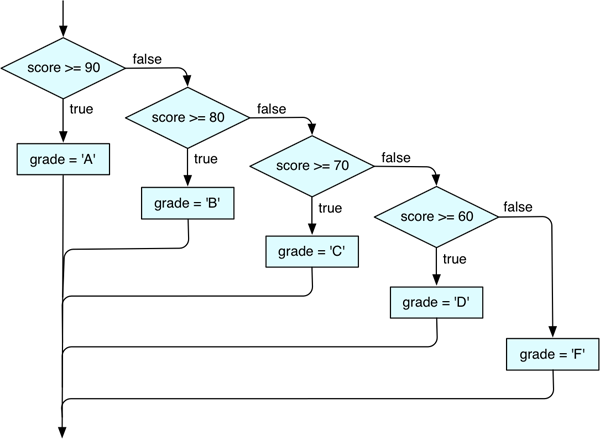
\includegraphics[width=.8\linewidth]{images/elseif.png}
    \end{center}
\end{frame}

\begin{frame}[fragile]{The \textbf{if...else if...else} Statement}{}
    \begin{block}{}
        To test multiple conditions, we can cascade if statements
    \end{block}
    \begin{minted}{c++}
        if (temperature >= 35) {
            cout << "Buy an ice ceam cone" << endl;
        }
        else if (temperature >= 25) {
            cout << "Buy a lollipop" << endl;
        }
        else if (temperature >= 15) {
            cout << "Buy a coffee" << endl;
        }
        else {
            cout << "Buy a sweater !" << endl;
        }
    \end{minted}
\end{frame}

\begin{frame}[fragile]{The \textbf{if...else if...else} Statement}{}
    \begin{itemize}
        \item The first statement must be an \emph{if}.
        \item After this, there can be any number of \emph{if else} statements. 
        \item At the end, there can be one (or zero) \emph{else} statement. 
    \end{itemize}
\end{frame}

\subsection{Nested Conditionals}
\begin{frame}[fragile]{Nested Conditionals}{}
    \begin{center}
        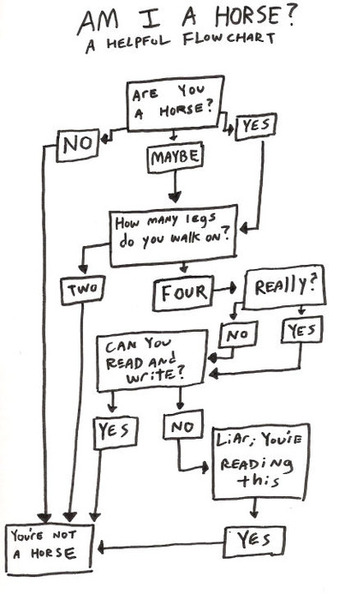
\includegraphics[width=.4\linewidth]{images/horse.jpg}
    \end{center}
\end{frame}

\begin{frame}[fragile]{Nested Conditionals}{}
    \begin{minted}{c++}
        if (temperature >= 35) {
            if (money >= 45) {
                cout << "Buy a Cornetto" << endl;
                money -= 45;
                if (money > 0) {
                    cout << "Buy a candy" << endl;
                }
                else
                    cout << "Out of Money :(" << endl;
            }
            else
                cout << "Buy a Pepsi" << endl;
        }
        else {
            cout << "Buy a lollipop" << endl;
        }
    \end{minted}
\end{frame}

\subsection{Exercises}

\begin{frame}[fragile]{Lab Time !}{Write programs for each of the following specifications}
    \begin{block}{~\vspace{0.5cm}}
    \begin{center}
    \vspace{-0.6cm}
    \begin{tabular}{p{0.45\textwidth}|p{0.45\textwidth}}
        \textcolor{white}{\bf Input} & \textcolor{white}{\bf Output} \\
        Four integers &
        Maximum and second max value \\ \hline
        Cutoff for A, B, C grades, and also marks of one student (out of 100) &
        1. Are the cutoffs valid ?\hfill\hspace{3em} 2. Student's grade (A,B,C) \\ \hline
        Three points (vertices of triangle) in terms of $(x,y)$ coordinates &
        Whether the triangle is equilateral, isosceles, or scalene
    \end{tabular}
    \end{center}
    \end{block}
    \begin{block}{}
        Write a program that takes as input, the coefficients of a quadratic equation
        ($Ax^2+Bx+C$), and outputs the roots (both real and imaginary).
    \end{block}
    \setbeamercolor{block title}{use=structure,fg=white,bg=red!35!black}
    \begin{block}{Sorting}
        Write a program that accepts $N$ numbers as input,
        and prints them out in ascending order.
    \end{block}
\end{frame}




\end{document}


